\section{Today's problem}
\label{sec:today_s_problem}

\begin{frame}
	\frametitle{Let's solve a problem!}
	\framesubtitle{Searching in a sorted list}
	
	\begin{columns}
		\column{0.455\textwidth}
	\begin{center}
		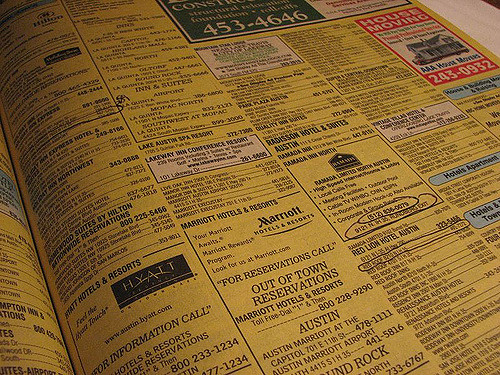
\includegraphics[width=0.9\textwidth]{figures/phonebook.jpg}\\
		\hspace*{15pt}\hbox{\scriptsize Image By:\thinspace{\itshape mk ecker}}
		% https://www.flickr.com/photos/93678621@N00/247922018/
	\end{center}
		\column{0.455\textwidth}
		\begin{questionblock}{I'm getting old}
			Who remembers these?
		\end{questionblock}
			
	\end{columns}
\end{frame}

\begin{frame}
	\frametitle{Let's solve a problem!}
	\framesubtitle{Searching in a sorted list}
	
	\begin{columns}
		\column{0.505\textwidth}
	\begin{center}
		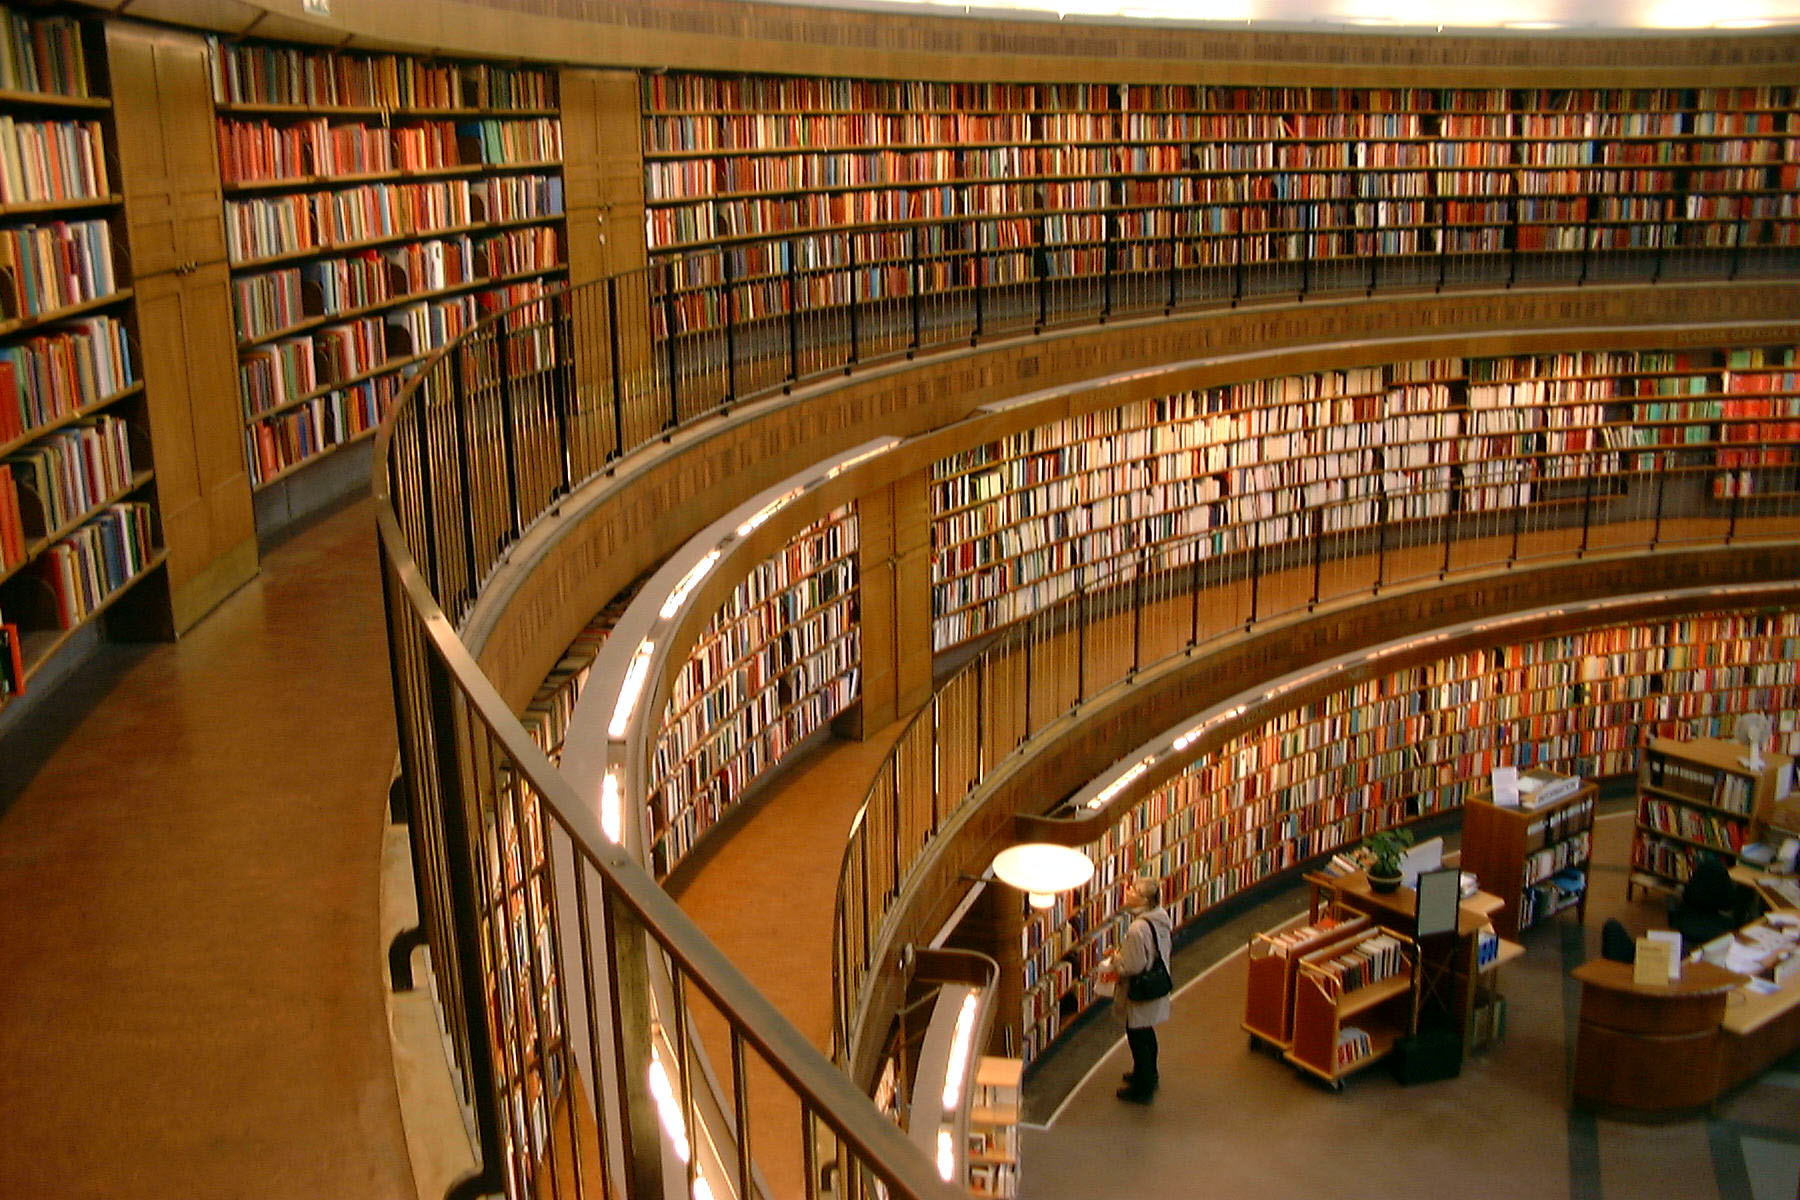
\includegraphics[width=0.9\textwidth]{figures/library.jpg}\\
		\hspace*{15pt}\hbox{\scriptsize Image By:\thinspace{\itshape Marcus Hansson}}
		% https://commons.wikimedia.org/wiki/File:Interior_view_of_Stockholm_Public_Library.jpg
	\end{center}
		\column{0.455\textwidth}
		\begin{questionblock}{Even for this}
			How do you look for books in a library? Say for instance you look for ``To kill a mockingbird'' by Harper Lee.
		\end{questionblock}
		\pause
		\begin{answerblock}{Well...}
			\begin{itemize}
				\item You see ``Split second'' by David Baldacci and you need to look further down the shelf.
					\pause
				\item You see ``The Amber Spyglass'' by Philip Pullman and you need to go back\dots
					\pause
				\item Let's formalise that idea!
			\end{itemize}
		\end{answerblock}
	\end{columns}
\end{frame}

\begin{frame}
	\frametitle{Recursion}
	\framesubtitle{Recursion}
	\begin{center}
		
\includegraphics[width=0.8\textwidth]{figures/google.png}\\
		\hspace*{15pt}\hbox{\scriptsize Source: Google}
	\end{center}	
\end{frame}

\begin{frame}
	\frametitle{Déjà Vu all over again?}
	
		\begin{block}{Recursion}
			A recursive function is a function that calls itself.
		\end{block}	
		\pause
		\begin{columns}
			\column{0.455\textwidth}
			\begin{exampleblock}{Fibonacci}
				For instance for Fibonacci:
				\begin{align*}
					F(1) &= 1 \\
					F(2) &= 1 \\
					F(n) &= F(n-1) + F(n-2) \text{ if $n > 2$}\\
				\end{align*}
			\end{exampleblock}
			\column{0.455\textwidth}
			\pause
		\lstinputlisting{code/fib.py}
				
		\end{columns}
\end{frame}

\section{Binary Search}
\label{sec:binary_search}


\begin{frame}
	\frametitle{Binary Search}
	\framesubtitle{Don't worry, there's no zeroes and ones involved}

	\begin{problemblock}{Binary search}
		Given a sorted list $L$, determine if it contains an item with value $v$.
	\end{problemblock}
	\pause
	\begin{exampleblock}{Example: Sorted names}
		\texttt{L = [Angelova, Chong, Hugtenburg, Sijm, van den Akker]}\\
		Does it contain \texttt{Sijm}?\\
		Answer: Yes!\\
		\pause
		\alert{But how do we get there?}
	\end{exampleblock}
	\pause
		\begin{alertblock}{Sublinear time}
			Remember that \texttt{in} from Python takes $\Theta(n)$ time. We want to improve on that!
		\end{alertblock}	
\end{frame}

\begin{frame}
	\frametitle{Binary search}
	\framesubtitle{The idea}
	
	\begin{overlayarea}{\textwidth}{\textheight}
		Let's build this algorithm:
		\pause
			\begin{columns}[t]
					
				\column{0.455\textwidth}
		\begin{enumerate}
			\scriptsize
			\only<6->{\item If the list is empty, return false}
		\item \only<6->{Otherwise\dots}Take the middle element of the list\only<7->{ with index \texttt{m}}, with value $x$.
		\item If $x = v$, return true.
		\pause
		\item If $x > v$, \alt<8->{return binary search in \texttt{L[:m]}.}{start looking in the \alt<5->{left}{\_\_\_} side of the list.} 
		\item If $x < v$, \alt<8->{return binary search in \texttt{L[m+1:]}.}{start looking in the \alt<5->{right}{\_\_\_} side of the list.}
		\end{enumerate}
				\column{0.605\textwidth}
		\only<11->{
			\lstinputlisting{code/binary-search.py}	
		}
			\end{columns}
		\only<4>{
			\begin{questionblock}{Filling in the blanks}
				\small
				What should we put on the blanks?
				\vspace*{-10pt}
				\begin{multicols}{2}
				\begin{enumerate}[A.]
					\item `left' on line 3 and `left' on line 4. 
					\item `left' on line 3 and `right' on line 4. 
					\item `right' on line 3 and `left' on line 4. 
					\item `right' on line 3 and `right' on line 4. 
					\item I don't know.
				\end{enumerate}	
			\end{multicols}
			\end{questionblock}
		}
		\only<9>{
			\begin{block}{Pseudocode}
				The above is what some might call \textit{pseudocode}. A natural language description of our program.			
			\end{block}	
		}
		\only<10>{
			\begin{exampleblock}{Let's do an example!}
				But just on the board, rather than in the slides.
			\end{exampleblock}	
		}
	\end{overlayarea}
\end{frame}

\begin{frame}
	\frametitle{So how well does this do?}

		\begin{block}{Reminder}
			Our time to beat is the Python built-in \texttt{in} operator that requires $\Theta(n)$ time!
		\end{block}	
		\begin{columns}
			\column{0.605\textwidth}
				\lstinputlisting{code/binary-search.py}	
			\column{0.405\textwidth}
			\pause
			\begin{questionblock}{T(n)}
				What is the runtime of this function? 
				Try to formulate a recursive $T(n)$, where $n$ is \texttt{len(L)}.
			\end{questionblock}	
			\pause
			\begin{answerblock}{T(n)}
				$T(0) = c_0$ for lines 5 and 6.\\
				$T(n) = T(\lfloor n/2 \rfloor) + c_1 + c_2n$ for lines 8 through 15.
			\end{answerblock}
		\end{columns}
\end{frame}

\begin{frame}
	\frametitle{So how well does this do? In terms of space}

		\begin{columns}
			\column{0.605\textwidth}
			\lstinputlisting{code/binary-search.py}	
			\column{0.405\textwidth}
			\begin{questionblock}{S(n)}
				What is the runtime of this function? 
				Try to formulate a recursive $S(n)$, where $n$ is \texttt{len(L)}.
			\end{questionblock}	
			\pause
			\begin{answerblock}{S(n)}
				$S(0) = c_0$ for lines 5 and 6.\\
				$S(n) = S(\lfloor n/2 \rfloor) + c_1 + c_2n$ for lines 8 through 15.
			\end{answerblock}
		\end{columns}
\end{frame}

\begin{frame}
	\frametitle{No improvements}
		\begin{block}{Reminder}
			Our time to beat is the Python built-in \texttt{in} operator that requires $\Theta(n)$ time!
		\end{block}	
		\begin{exampleblock}{Making it strictly better}
			This is still $O(n)$ at least... Because we make copies of the list in lines 13 and 14.	\\
			How about we two more parameters: lowest index, largest index instead of a copy of half of the list.\\
			Now we only have $T(n) = T(n/2) + c_1$.
		\end{exampleblock}	
\end{frame}

\begin{frame}
	\frametitle{How do we solve this?}

	\begin{questionblock}{Recurrence Equations}
		How do we get to $O(...)$ now?
	\end{questionblock}
	\pause
	\begin{answerblock}{Repeated unfolding}
		$T(n) = T(n/2) +c_1$, so $T(n/2) = T(n/4) + c_1$.\\
		Substituting this, we get: $T(n) = T(n/4) + 2c_1$.
	\end{answerblock}
	\pause
	\begin{alertblock}{As a computer scientist...}
		To make the math a little `cleaner' we will assume $n = 2^m$ for some integer $m \geq 0$.	
	\end{alertblock}
\end{frame}

\begin{frame}
	\frametitle{Solving it: getting a closed form}

	Repeated unfolding:
	\begin{align*}
		T(n) &= T(\lfloor n/2 \rfloor) + c_1\\
				 &= T(\lfloor n/4 \rfloor) + 2c_1\\
				 &= T(\lfloor n/8 \rfloor) + 3c_1\\
				 &= T(\lfloor n/2^k \rfloor) + kc_1\\
		\intertext{Take $k= \log_2(n+1)$ to get to $T(0)$}
		     &= T(\lfloor n/2^{\log_2(n+1)} \rfloor) + c_1\log_2(n+1)\\
				 &= T(0) + c_1\log_2(n+1)\\
				 &= c_0 + c_1\log_2(n+1)
	\end{align*}
\end{frame}

\begin{frame}
	\frametitle{Confirming our `repeated unfolding'}
	\begin{questionblock}{How do we know it works?}
		How do we know this `guess' is correct?	
	\end{questionblock}
	\begin{answerblock}{Induction!}
		Induction! (Let's see what you think of my idea of induction ;))
	\end{answerblock}
\end{frame}

\begin{frame}
	\frametitle{Proof by induction}
	\framesubtitle{For powers of 2}
	\begin{proof}
		To prove: $T(n) = c_0 + c_1 \log_2(n)$ for $T(n)= \begin{cases}
			c_0 & \text{ if n = 1}\\
			T(n/2) + c_1 & \text{ else}
		\end{cases}$.	\\
		Base case ($n=0$): $T(0) = c_0 = c_0 + c_1 \cdot 0 = c_0 + c_1\log_2(0+1)$.\\
		Inductive case:
		Assume for arbitrary $k$: $T(k) = c_0 + c_1 \log_2(k+1)$. (IH)\\
		\vspace*{-15pt}
		\begin{align*}
			T(2k) &= T(2k/2) + c_1\\
					 &= T(k) + c_1\\
					 &=_\text{\small IH} c_0 + c_1\log_2(k+1) + c_1\\
					 &= c_0 + c_1(\log_2(k+1) + \log_2(2))\\
					 &= c_0 + c_1(\log_2(2(k+1)))
		\end{align*}
		Since $k$ was arbitrarily chosen, it holds for all $n \geq 0$.
	\end{proof}
\end{frame}

\begin{frame}
	\frametitle{So...}
		\begin{exampleblock}{Main take-away}
			Searching in an unsorted list: $O(n)$.\\
			Searching in an sorted list: $O(\log(n))$.
		\end{exampleblock}	
		\pause
		\begin{questionblock}{So\dots}
			Does that mean we should always sort our list?
		\end{questionblock}
		\pause
		\begin{answerblock}{It depends}
			It depends\dots\\
			We will find out when we discuss sorting in week 3!
		\end{answerblock}
\end{frame}
